\newcommand\bax{
  \begin{center}
    \begin{tikzpicture}[scale=0.85]
      % horizontal extent ensures left edge at x=-5 aligns with structure below
      \draw[->] (-5,0) -- (5,0) node[above right] {$x$};
      \draw[->] (-5,-1.1) -- (-5,1.1) node[left] {$B_z$};
      \draw[dashed,gray] (-5,0) -- (5,0);
    \end{tikzpicture}
  \end{center}
}

\begin{activity}{Magnetic Structures}

\section*{Purpose}

This activity mirrors previous gravity workshops. You will reason about magnetic anomaly shapes and compare them directly with gravity anomalies from the same structures.

\section*{Learning Outcomes}

By the end of this activity, you should be able to:
\begin{itemize}
  \item Sketch the expected vertical magnetic anomaly for a range of simple geological structures.
  \item Identify the sign, symmetry, width, location of steepest gradients, and asymptotic behavior for each structure.
  \item Compare magnetic and gravity anomalies for the same body and explain key differences in terms of the dipolar nature of magnetic fields.
  \item Explain why magnetic interpretation is more non-unique than gravity interpretation.
\end{itemize}

Assume:
\begin{itemize}
  \item Uniform susceptibility
  \item Induced magnetisation only
  \item Constant inducing field
\end{itemize}

\section*{Background}

Before sketching, it's worth anticipating one basic difference between gravity and magnetic fields from a compact source. Stripped down to the geometry alone --- dropping mass, susceptibility, and other physical constants --- the two fields scale with distance $r$ from the source as
\[
    g \;\propto\; \frac{1}{r^2}
    \qquad\qquad
    B \;\propto\; \frac{1}{r^3}.
\]
A magnetic field falls off one power of $r$ faster than the equivalent gravity field, because every magnetic source has both a positive and a negative pole rather than a single sign of mass. Practically, this means a magnetic anomaly from a compact, near-surface source should look \emph{narrower and more sharply peaked} than a gravity anomaly from a source of the same size and depth. The same one-power-faster relationship holds for extended sources too, such as the cylinder and slabs below, even though the exact exponents shift with source geometry.

\section*{Instructions}

For each structure:
\begin{enumerate}
  \item Sketch the expected vertical magnetic anomaly
  \item Indicate sign, symmetry, width, and strongest gradients
  \item State how it differs from the gravity anomaly
\end{enumerate}

\section*{Structures}

% ==========================================================
% A) Buried Cylinder
% ==========================================================
\begin{center}
\textbf{A) Buried Cylinder (2D; infinite strike)}
\end{center}

\bax

\begin{center}
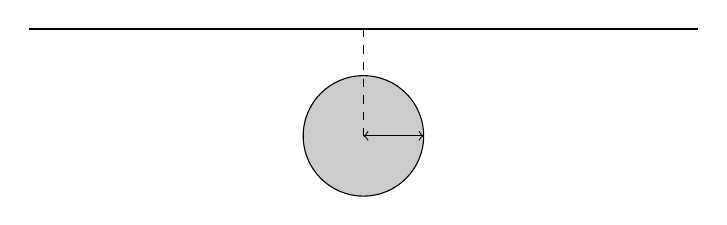
\begin{tikzpicture}[scale=0.85]
  \draw[thick] (-5,0) -- (5,0); % surface only
  % Sphere
  \def\xc{0} \def\zc{-1.6} \def\r{0.9}
  \draw[fill=gray!40] (\xc,\zc) circle (\r);
  \draw[dashed] (\xc,0) -- (\xc,\zc);
  \draw[<->] (\xc+\r,\zc) -- (\xc,\zc);
\end{tikzpicture}
\end{center}

\bigskip\bigskip

% ==========================================================
% B) Vertical Slab
% ==========================================================
\begin{center}
\textbf{B) Vertical Slab}
\end{center}

\bax

\begin{center}
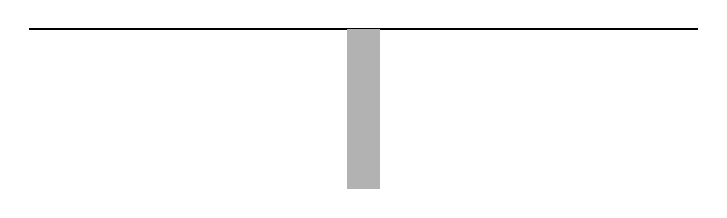
\begin{tikzpicture}[scale=0.85]
  \draw[thick] (-5,0) -- (5,0);
  \fill[gray!60] (-0.25,0) rectangle (0.25,-2.4);
\end{tikzpicture}
\end{center}

\bigskip\bigskip

% ==========================================================
% C) Finite-Extent Sill
% ==========================================================
\begin{center}
\textbf{C) Finite-Extent Horizontal Slab}
\end{center}

\bax

\begin{center}
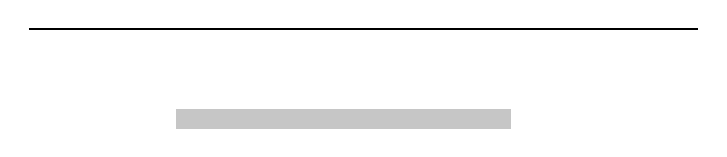
\begin{tikzpicture}[scale=0.85]
  \draw[thick] (-5,0) -- (5,0);
  \fill[gray!45] (-2.8,-1.2) rectangle (2.2,-1.5);
\end{tikzpicture}
\end{center}

\bigskip\bigskip

% ==========================================================
% D) Semi-Infinite Horizontal Slab
% ==========================================================
\begin{center}
\textbf{D) Semi-Infinite Horizontal Slab}
\end{center}

\bax

\begin{center}
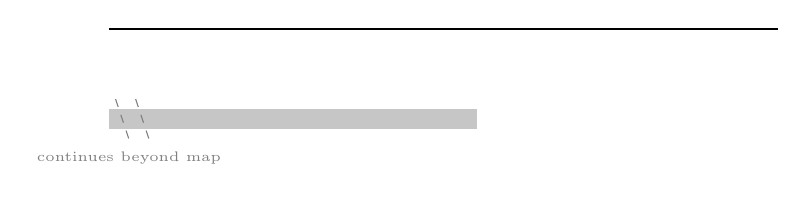
\begin{tikzpicture}[scale=0.85]
  \draw[thick] (-5,0) -- (5,0);
  \fill[gray!45] (-5,-1.2) rectangle (0.5,-1.5);
  % break marks at the frame edge signal the slab continues beyond the map
  \draw[gray, dashed] (-4.9,-1.05) -- (-4.7,-1.65);
  \draw[gray, dashed] (-4.6,-1.05) -- (-4.4,-1.65);
  \node[font=\tiny, gray, below] at (-4.7,-1.7) {continues beyond map};
\end{tikzpicture}
\end{center}

\bigskip

\begin{questions}
  \question{Vertical vs Horizontal Inducing Field}
  Repeat one case assuming a horizontal inducing field.

  \begin{enumerate}
    \item How does the anomaly shape change?
    \answerbox[2cm]
    \item Which case appears more gravity-like?
    \answerbox[2cm]
    \item Why does gravity not behave this way?
    \answerbox[2cm]
  \end{enumerate}

  \question{Reflection}
  Give two reasons why magnetic interpretation is more non-unique than gravity.

  \answerbox[3cm]
\end{questions}

\section*{Key Ideas}

\textbf{Sign and shape depend on source geometry and field direction, not just on source strength.} A mass excess always produces a positive gravity anomaly, full stop. A susceptibility contrast produces a magnetic anomaly whose sign and shape depend on the body's geometry \emph{and} on the direction of the inducing field --- at the magnetic pole a symmetric body gives a symmetric, bipolar anomaly; at lower latitudes the same body gives an asymmetric one with shifted lobes. Gravity has no equivalent to either effect. (Recall the monopole/dipole comparison from Activity 6.A, Figure~\ref{fig:polar}.)

\textbf{Finite structures produce edge effects the end-member sketches don't show.} Near the single edge of Structure D, the anomaly peaks just inside the edge and dips to a trough just outside it, then returns fully to zero further away --- a point near the edge sits closer to source material on one side than the other, the same near-vs-far dipole reasoning behind the $1/r^3$ falloff above, just applied across an extended source. Structure C has \emph{two} such edges. If they're far enough apart, each produces its own peak-and-trough and the interior settles to a shallow minimum rather than true zero; if they're close together, the two signatures can merge into something that looks more like a single smooth bump. Compare your sketches for C and D directly --- can you tell which regime C is in?

\textbf{Non-uniqueness is greater in magnetics than gravity.} Three unknowns --- susceptibility, geometry, and magnetisation direction --- must all be constrained simultaneously. Remanent magnetisation (a frozen-in field direction different from today's) adds a fourth unknown. Additional constraints from geology, paleomagnetism, or other data are usually required to discriminate between models.

\end{activity}